\documentclass[12pt,a4paper]{report}

% -------------------------------------------------
% LANGUE ET ENCODAGE
% -------------------------------------------------
\usepackage[T1]{fontenc}
\usepackage[utf8]{inputenc}
\usepackage[french]{babel}
\usepackage{lmodern}
\usepackage{microtype}

% Mathématiques et algorithmes
\usepackage{amsmath,amssymb}
\usepackage{algorithm}
\usepackage{algpseudocode}

% Tableaux et mise en page
\usepackage{array}
\usepackage{multirow}
\usepackage{makecell}
\usepackage{xcolor}
\usepackage{caption}
\usepackage{subcaption}

% Code source et JSON
\usepackage{listings}
\usepackage{upquote}

% Graphiques et diagrammes
\usepackage{tikz}
\usetikzlibrary{
    arrows.meta,
    positioning,
    shapes.geometric,
    shapes.multipart,
    fit,
    backgrounds,
    calc
}

% Liens et références
\usepackage{url}

% -------------------------------------------------
% MISE EN PAGE
% -------------------------------------------------
\usepackage[a4paper,margin=2.4cm,headheight=15pt]{geometry}
\usepackage{setspace}
\usepackage{fancyhdr}

\setlength{\parskip}{5pt}
\setlength{\parindent}{0pt}
\onehalfspacing

% -------------------------------------------------
% IMAGES ET FIGURES
% -------------------------------------------------
\usepackage{graphicx}
\usepackage{float}
\usepackage{caption}
\usepackage{subcaption}

% Chemins des images
\graphicspath{
    {img/}
    {seif/}
    {yassine/}
    {raslen/}
}

% -------------------------------------------------
% TABLEAUX
% -------------------------------------------------
\usepackage{booktabs}
\usepackage{array}
\usepackage{tabularx}
\usepackage{multirow}
\usepackage{longtable}

\newcolumntype{Y}{>{\raggedright\arraybackslash}X}

% -------------------------------------------------
% MATHEMATIQUES ET UNITES
% -------------------------------------------------
\usepackage{amsmath}
\usepackage{siunitx}

\sisetup{
    locale=FR,
    per-mode=symbol
}

% -------------------------------------------------
% DIAGRAMMES ET GRAPHIQUES
% -------------------------------------------------
\usepackage{tikz}
\usepackage{pgfplots}

\pgfplotsset{compat=1.18}

\usetikzlibrary{
    arrows.meta,
    positioning,
    shapes.geometric,
    fit,
    calc
}

% -------------------------------------------------
% COULEURS
% -------------------------------------------------
\usepackage{xcolor}

\definecolor{bleu}{RGB}{20,55,95}
\definecolor{griscode}{RGB}{246,247,249}
\definecolor{bleuclaire}{RGB}{225,235,245}

% -------------------------------------------------
% CODE SOURCE
% -------------------------------------------------
\usepackage{listings}

\lstset{
    basicstyle=\ttfamily\small,
    backgroundcolor=\color{griscode},
    frame=single,
    breaklines=true,
    columns=fullflexible,
    showstringspaces=false,
    captionpos=b
}

% -------------------------------------------------
% LISTES
% -------------------------------------------------
\usepackage{enumitem}

% -------------------------------------------------
% HYPERLIENS ET METADONNEES PDF
% -------------------------------------------------
\usepackage[hidelinks]{hyperref}

\hypersetup{
    colorlinks=true,
    linkcolor=bleu,
    urlcolor=bleu,
    citecolor=bleu,
    pdftitle={Classification et Filtrage Bayésien},
    pdfauthor={Lamouchi Seif, ElJenzri Yassine, Moussa Raslen},
    pdfsubject={TNS}
}

% -------------------------------------------------
% EN-TETE ET PIED DE PAGE
% -------------------------------------------------
\pagestyle{fancy}
\fancyhf{}

\lhead{Classification et Filtrage Bayésien}
\rhead{TNS}
\cfoot{\thepage}


% -------------------------------------------------
% COMMANDES PERSONNALISEES
% -------------------------------------------------

% Placeholder pour une figure ou un diagramme
\newcommand{\figureplaceholder}[2]{
    \begin{figure}[H]
        \centering
        \IfFileExists{#1}{
            \includegraphics[width=.96\textwidth,
            height=.58\textheight,
            keepaspectratio]{#1}
        }{
            \fbox{
                \parbox{.88\textwidth}{
                    \centering
                    \vspace{1cm}
                    \textbf{Figure à ajouter :} \texttt{#1}
                    \vspace{1cm}
                }
            }
        }
        \caption{#2}
    \end{figure}
}

% Marqueur temporaire pour les éléments à compléter
\newcommand{\todo}[1]{
    \textit{\textcolor{red}{[À compléter : #1]}}
}


\begin{document}


% Couleur principale
\definecolor{bleu}{RGB}{0, 70, 140}

\pagenumbering{gobble}

\begin{titlepage}
\centering

% Logos institutionnels
\noindent
\begin{minipage}[c]{0.46\textwidth}
    \centering
    \IfFileExists{universite-de-carthage.png}
    {
\includegraphics[height=4cm,keepaspectratio]{universite-de-carthage.png}}
    {\fbox{\parbox[c][2.2cm][c]{0.88\linewidth}{\centering Logo\\Université de Carthage}}}
\end{minipage}
\hfill
\begin{minipage}[c]{0.46\textwidth}
    \centering
    \IfFileExists{logo-insat.jpg}
    {
\includegraphics[height=3.5cm,keepaspectratio]{logo-insat.jpg}}
    {\fbox{\parbox[c][2cm][c]{0.88\linewidth}{\centering Logo\\INSAT}}}
\end{minipage}

\par\vspace{.2cm}

{\large Ministère de l'Enseignement Supérieur et de la Recherche Scientifique\par}


{\large Université de Carthage\par}


{\large Institut National des Sciences Appliquées et de Technologie (INSAT)\par}

{\color{bleu}\rule{\textwidth}{1.3pt}}
\vspace{.1cm}

{\Huge\bfseries Compte Rendu TP3 \par}
\vspace{.2cm}

{\LARGE \par}
Traitement Numérique des Signaux (TNS) \par
\vspace{.1cm}

{\color{bleu}\rule{\textwidth}{1.3pt}}

\vspace{.65cm}

{\huge\bfseries
Classification et filtrage bayésien
\par}


\vspace{.75cm}

{\Large\textbf{Réalisé par}\par}
\vspace{.25cm}

{\Large Lamouchi Seif\par}
\vspace{.08cm}
{\Large EL Jenzri Yassine\par}
\vspace{.08cm}
{\Large Moussa Raslene\par}

\vfill

\begin{tabular}{rl}
\textbf{Matière :} & TNS\\
\textbf{Niveau :} & Cycle ingénieur -- RT4 \\
\textbf{Encadrant :} & Mme Rim Amara Boujemaa\\
\textbf{Année universitaire :} & 2026--2027
\end{tabular}

\vspace{.45cm}

\end{titlepage}

\clearpage
\pagenumbering{arabic}


\tableofcontents
\listoffigures
\listoftables


% Fichier : latex/yassine/yassine.tex
% Ce fichier est un fragment à intégrer dans le rapport principal avec :
% 
% Fichier : latex/yassine/yassine.tex
% Ce fichier est un fragment à intégrer dans le rapport principal avec :
% 
% Fichier : latex/yassine/yassine.tex
% Ce fichier est un fragment à intégrer dans le rapport principal avec :
% \input{yassine/yassine}
% Ne pas ajouter de \documentclass, \begin{document} ou \end{document} ici.

\chapter{Motifs des classes et étude de DiffWave}

\section{Construction des motifs des classes}

\subsection{Objectif et modèle du signal}

L'objectif de cette partie est de construire les deux classes de symboles, notées $E^+$ et $E^-$, puis d'étudier leur représentation dans l'espace des observations. Le symbole courant prend l'une des deux valeurs :
\[
d(n)\in\{-1,+1\}.
\]

Le signal reçu est modélisé par la convolution du signal transmis avec la réponse impulsionnelle du canal, à laquelle s'ajoute un bruit :
\begin{equation}
x(n)=\sum_{i=0}^{M-1}c(i)d(n-i)+w(n),
\end{equation}
où $c(i)$ représente les coefficients du canal, $d(n)$ les symboles transmis et $w(n)$ le bruit additif.

Les paramètres utilisés sont :
\[
M=2,\qquad P=2,\qquad c(0)=1,\qquad c(1)=0.5.
\]
Le vecteur d'observation contient deux échantillons successifs :
\[
X(n)=
\begin{pmatrix}
x(n)\\
x(n-1)
\end{pmatrix}.
\]

\subsection{Construction de la matrice de convolution}

Pour calculer les deux composantes de $X(n)$, nous considérons le vecteur des symboles :
\[
D(n)=
\begin{pmatrix}
d(n)\\
d(n-1)\\
d(n-2)
\end{pmatrix}.
\]

En absence de bruit, la relation matricielle s'écrit :
\begin{equation}
X(n)=CC\,D(n),
\end{equation}
avec :
\begin{equation}
CC=
\begin{pmatrix}
c(0)&c(1)&0\\
0&c(0)&c(1)
\end{pmatrix}
=
\begin{pmatrix}
1&0.5&0\\
0&1&0.5
\end{pmatrix}.
\end{equation}

La première ligne donne $x(n)=d(n)+0.5d(n-1)$, tandis que la deuxième donne $x(n-1)=d(n-1)+0.5d(n-2)$. La matrice $CC$ traduit donc l'effet du canal sur les symboles courant et passés.

\subsection{Détermination des quatre motifs de chaque classe}

La classe $E^+$ correspond à $d(n)=+1$ et la classe $E^-$ à $d(n)=-1$. Les deux symboles précédents, $d(n-1)$ et $d(n-2)$, peuvent chacun prendre les valeurs $-1$ ou $+1$. Il existe donc $2^2=4$ combinaisons par classe, soit huit motifs au total.

Les coordonnées sont calculées à partir de $X(n)=CC\,D(n)$.

\begin{table}[H]
\centering
\caption{Motifs théoriques de la classe $E^+$ sans bruit}
\label{tab:yassine-motifs-plus}
\begin{tabular}{ccccc}
\toprule
$d(n)$ & $d(n-1)$ & $d(n-2)$ & $x(n)$ & $x(n-1)$\\
\midrule
$+1$ & $+1$ & $+1$ & $1.5$ & $1.5$\\
$+1$ & $+1$ & $-1$ & $1.5$ & $0.5$\\
$+1$ & $-1$ & $+1$ & $0.5$ & $-0.5$\\
$+1$ & $-1$ & $-1$ & $0.5$ & $-1.5$\\
\bottomrule
\end{tabular}
\end{table}

\begin{table}[H]
\centering
\caption{Motifs théoriques de la classe $E^-$ sans bruit}
\label{tab:yassine-motifs-moins}
\begin{tabular}{ccccc}
\toprule
$d(n)$ & $d(n-1)$ & $d(n-2)$ & $x(n)$ & $x(n-1)$\\
\midrule
$-1$ & $+1$ & $+1$ & $-0.5$ & $1.5$\\
$-1$ & $+1$ & $-1$ & $-0.5$ & $0.5$\\
$-1$ & $-1$ & $+1$ & $-1.5$ & $-0.5$\\
$-1$ & $-1$ & $-1$ & $-1.5$ & $-1.5$\\
\bottomrule
\end{tabular}
\end{table}

\subsection{Résultats en absence de bruit}

\begin{figure}[H]
\centering
\IfFileExists{../figures/01_classes_sans_bruit.png}{
    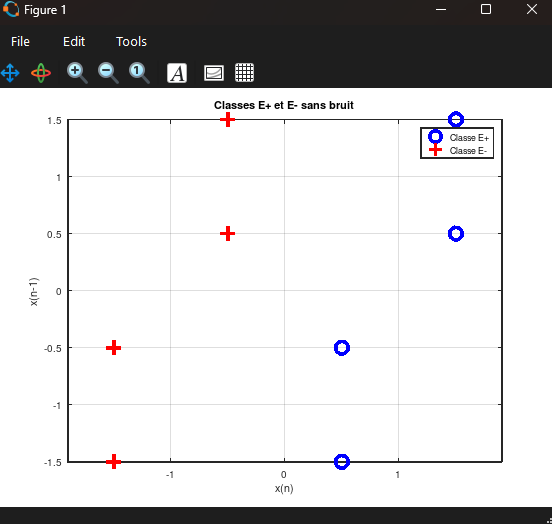
\includegraphics[width=0.82\textwidth]{../figures/01_classes_sans_bruit.png}
}{
    \fbox{\parbox{0.78\textwidth}{\centering Figure à ajouter : \texttt{01\_classes\_sans\_bruit.png}}}
}
\caption{Représentation des motifs des classes $E^+$ et $E^-$ sans bruit.}
\label{fig:yassine-sans-bruit}
\end{figure}

La figure~\ref{fig:yassine-sans-bruit} présente les huit motifs théoriques calculés à partir de la matrice $CC$. Chaque point correspond à une combinaison des trois symboles $d(n)$, $d(n-1)$ et $d(n-2)$. En absence de bruit, les observations prennent exactement les coordonnées calculées dans les tableaux précédents : aucune dispersion aléatoire n'est présente.

Cette figure constitue la référence pour l'étude du bruit. Elle permet de comparer les positions idéales des motifs avec les observations perturbées dans les expériences suivantes.

\subsection{Modélisation du bruit gaussien}

Nous ajoutons aux observations un bruit gaussien centré :
\[
W(n)\sim\mathcal{N}(0,\sigma^2 I_P),
\]
où $\sigma^2$ est la variance du bruit et $I_P$ la matrice identité de dimension $P$.

Les observations bruitées s'écrivent :
\begin{equation}
X_{\mathrm{bruité}}(n)=CC\,D(n)+W(n).
\end{equation}

Dans le programme Octave, les composantes du bruit sont générées avec \texttt{randn}, puis multipliées par $\sqrt{\sigma^2}$ afin d'obtenir la variance souhaitée. La simulation utilise $N=100$ observations par motif. Les variances $0.01$, $0.2$ et $1.0$ sont des valeurs choisies pour illustrer l'effet progressif du bruit ; elles ne constituent pas des valeurs imposées par l'énoncé.

\subsection{Analyse des résultats avec bruit}

\begin{figure}[H]
\centering
\IfFileExists{../figures/02_classes_bruit_variance_0_01.png}{
    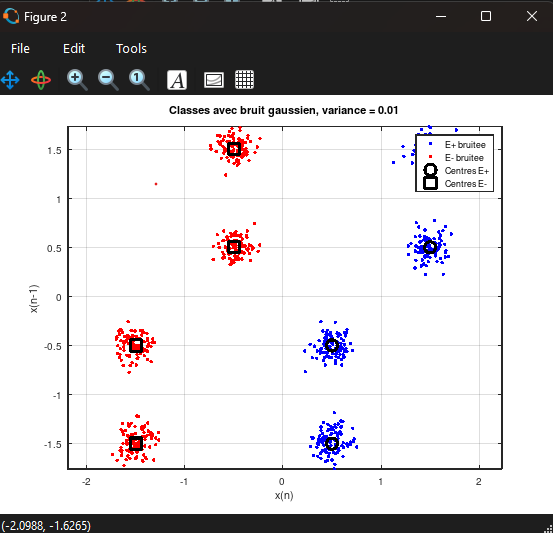
\includegraphics[width=0.82\textwidth]{../figures/02_classes_bruit_variance_0_01.png}
}{
    \fbox{\parbox{0.78\textwidth}{\centering Figure à ajouter : \texttt{02\_classes\_bruit\_variance\_0\_01.png}}}
}
\caption{Observations bruitées pour une variance $\sigma^2=0.01$.}
\label{fig:yassine-bruit-faible}
\end{figure}

Pour $\sigma^2=0.01$, le bruit est faible. Les observations restent généralement proches des positions théoriques de la figure~\ref{fig:yassine-sans-bruit}. La dispersion autour des motifs est limitée et les deux classes conservent une séparation visuelle nette. Le bruit modifie légèrement les coordonnées, sans perturber fortement la structure des classes.

\begin{figure}[H]
\centering
\IfFileExists{../figures/03_classes_bruit_variance_0_2.png}{
    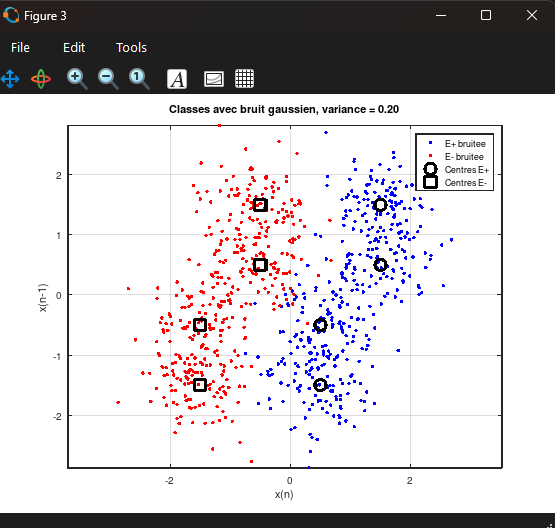
\includegraphics[width=0.82\textwidth]{../figures/03_classes_bruit_variance_0_2.png}
}{
    \fbox{\parbox{0.78\textwidth}{\centering Figure à ajouter : \texttt{03\_classes\_bruit\_variance\_0\_2.png}}}
}
\caption{Observations bruitées pour une variance $\sigma^2=0.2$.}
\label{fig:yassine-bruit-moyen}
\end{figure}

Lorsque la variance augmente à $\sigma^2=0.2$, l'amplitude typique des perturbations devient plus importante. Les nuages de points sont davantage étalés autour des motifs théoriques. La distinction entre les classes est donc moins évidente que dans le cas du bruit faible, même si les observations restent globalement organisées autour de leurs positions théoriques.

\begin{figure}[H]
\centering
\IfFileExists{../figures/04_classes_bruit_variance_1_0.png}{
    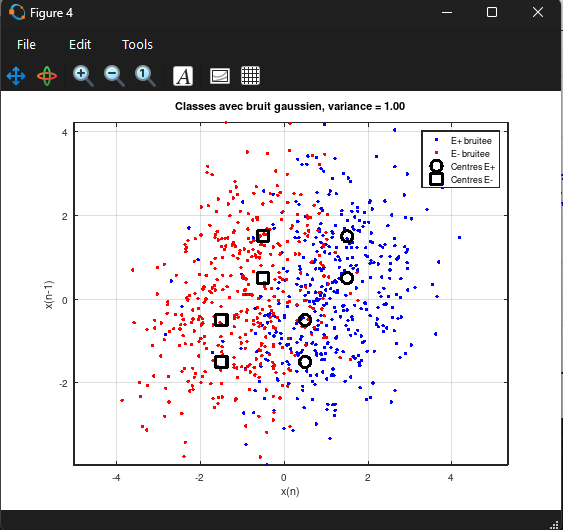
\includegraphics[width=0.82\textwidth]{../figures/04_classes_bruit_variance_1_0.png}
}{
    \fbox{\parbox{0.78\textwidth}{\centering Figure à ajouter : \texttt{04\_classes\_bruit\_variance\_1\_0.png}}}
}
\caption{Observations bruitées pour une variance $\sigma^2=1.0$.}
\label{fig:yassine-bruit-fort}
\end{figure}

Pour $\sigma^2=1.0$, le bruit est important. Les observations peuvent s'éloigner sensiblement de leurs positions théoriques et les nuages deviennent plus dispersés. Des observations appartenant à des classes différentes peuvent alors se rapprocher, voire se chevaucher localement. La distinction entre les classes devient plus difficile et le risque d'erreur de classification augmente.

\begin{figure}[H]
\centering
\IfFileExists{../figures/05_comparaison_niveaux_bruit.png}{
    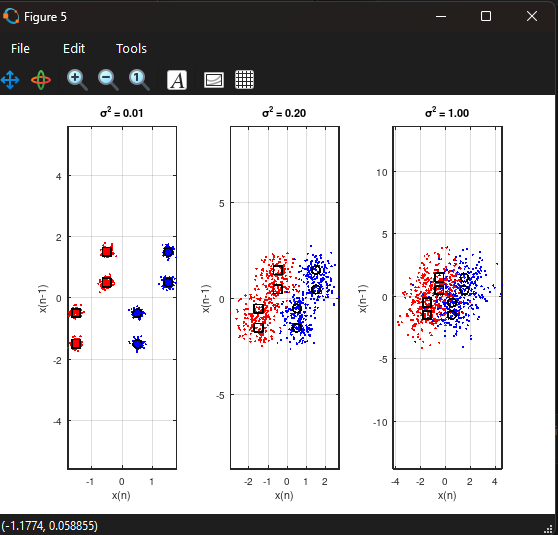
\includegraphics[width=0.90\textwidth]{../figures/05_comparaison_niveaux_bruit.png}
}{
    \fbox{\parbox{0.82\textwidth}{\centering Figure à ajouter : \texttt{05\_comparaison\_niveaux\_bruit.png}}}
}
\caption{Comparaison des observations pour les trois niveaux de bruit étudiés.}
\label{fig:yassine-comparaison-bruit}
\end{figure}

La comparaison met en évidence l'effet direct de la variance sur la dispersion des observations. Lorsque $\sigma^2$ augmente, les points s'écartent davantage de leurs positions idéales. La séparation visuelle des classes se dégrade progressivement, ce qui explique pourquoi une classification fiable devient plus difficile en présence d'un bruit important.

\subsection{Bilan de la partie 1.1}

La matrice de convolution $CC$ permet de représenter l'effet du canal sur les symboles transmis. Pour $M=2$ et $P=2$, les deux valeurs possibles du symbole courant définissent deux classes, et les deux symboles précédents conduisent à quatre motifs par classe.

Sans bruit, les motifs occupent leurs positions théoriques. L'ajout d'un bruit gaussien entraîne une dispersion autour de ces positions. Les simulations montrent que cette dispersion augmente avec la variance du bruit et peut rendre les classes plus difficiles à distinguer. Cette observation justifie l'intérêt d'un classifieur capable de prendre en compte les distributions statistiques des observations, comme le classifieur bayésien étudié dans la suite du TP.

\section{DiffWave : critère d'apprentissage, latence et mémoire}

\subsection{Principe général}

DiffWave est un modèle génératif fondé sur la diffusion, conçu pour produire des formes d'onde audio. Le processus direct ajoute progressivement du bruit à un signal audio réel jusqu'à obtenir un signal proche d'un bruit gaussien. Le processus inverse apprend à retirer progressivement ce bruit afin de reconstruire un signal audio plausible.

Pendant l'apprentissage, le réseau est entraîné sur des signaux perturbés à différents niveaux de diffusion. Il reçoit le signal bruité et l'indice de l'étape de diffusion, puis apprend à estimer le bruit qui a été ajouté.

\subsection{Critère de coût utilisé pendant l'apprentissage}

Une formulation courante de l'objectif d'apprentissage consiste à minimiser l'erreur quadratique entre le bruit réellement ajouté et le bruit estimé par le réseau :
\begin{equation}
\mathcal{L}(\theta)=
\mathbb{E}_{x_0,\epsilon,t}
\left[
\left\|
\epsilon-\epsilon_\theta(x_t,t)
\right\|_2^2
\right],
\end{equation}
où :
\begin{itemize}
    \item $x_0$ est le signal audio original ;
    \item $t$ est l'indice de l'étape de diffusion ;
    \item $\epsilon$ est le bruit gaussien ajouté ;
    \item $x_t$ est le signal perturbé à l'étape $t$ ;
    \item $\epsilon_\theta(x_t,t)$ est le bruit prédit par le réseau paramétré par $\theta$.
\end{itemize}

Le réseau cherche à produire une estimation du bruit aussi proche que possible du bruit réellement injecté. En apprenant à estimer ce bruit à différents niveaux de perturbation, il apprend indirectement à effectuer le processus inverse de diffusion.

L'article original de DiffWave présente un cadre probabiliste de diffusion et un objectif d'apprentissage lié à la borne variationnelle. La prédiction du bruit avec une erreur quadratique est une formulation pratique couramment utilisée pour entraîner ce type de modèle. Cette fonction de coût ne mesure pas directement la qualité audio finale : elle mesure l'écart entre le bruit réel et le bruit estimé pendant l'apprentissage.

\subsection{Latence et temps de génération}

La latence désigne le temps nécessaire pour générer le signal audio. Dans un modèle de diffusion, la génération nécessite plusieurs étapes successives du processus inverse. À chaque étape, le réseau estime le bruit et permet de produire un signal progressivement plus structuré.

Le temps de génération dépend principalement :
\begin{itemize}
    \item du nombre d'étapes de diffusion utilisées pendant l'inférence ;
    \item de la longueur du signal audio à générer ;
    \item de la taille et de la complexité du réseau ;
    \item du matériel utilisé, notamment du processeur ou du GPU ;
    \item de l'optimisation logicielle et de la précision numérique.
\end{itemize}

DiffWave est non autorégressif : il n'a pas besoin de prédire chaque échantillon audio en s'appuyant séquentiellement sur les échantillons précédents, comme le font les modèles autorégressifs classiques. Les opérations sur les positions temporelles d'une étape peuvent être réalisées en parallèle. En revanche, les étapes successives du processus inverse de diffusion restent dépendantes les unes des autres.

Augmenter le nombre d'étapes de diffusion peut améliorer la qualité de la génération, mais augmente généralement le temps de calcul. Il existe donc un compromis entre qualité audio et latence. Une valeur précise doit être mesurée sur une machine et avec une configuration données ; aucune mesure locale n'est avancée dans ce rapport.

\subsection{Consommation mémoire}

La consommation mémoire correspond à la quantité de mémoire vive ou de mémoire GPU nécessaire au chargement et à l'exécution du modèle. Elle dépend notamment :
\begin{itemize}
    \item du nombre de paramètres du réseau ;
    \item du nombre de canaux et de blocs internes de l'architecture ;
    \item de la longueur des séquences audio traitées ;
    \item de la taille du lot (\textit{batch size}) ;
    \item de la précision numérique utilisée ;
    \item du mode d'exécution : apprentissage ou inférence.
\end{itemize}

Pendant l'apprentissage, la consommation mémoire est généralement plus importante, car il faut conserver les activations intermédiaires nécessaires à la rétropropagation du gradient, en plus des paramètres et des états de l'optimiseur.

Pendant l'inférence, le calcul du gradient n'est pas nécessaire. La mémoire requise est donc généralement plus faible, même si elle reste influencée par la taille du modèle et la longueur audio générée.

Il faut distinguer la taille du fichier contenant les poids pré-entraînés de la mémoire réellement utilisée à l'exécution. Le chargement du modèle, les activations intermédiaires, les tampons de calcul et les données audio peuvent nécessiter davantage de mémoire que le seul fichier des poids.

\subsection{Synthèse de l'étude de DiffWave}

Le critère d'apprentissage de DiffWave vise à rapprocher le bruit prédit par le réseau du bruit réellement ajouté au signal. La latence dépend notamment du nombre d'étapes de diffusion, de la longueur audio et du matériel disponible. La mémoire dépend de l'architecture, des dimensions des données et du mode d'exécution.

Ces trois critères sont liés : une configuration plus coûteuse en calcul ou en mémoire peut permettre une génération de meilleure qualité, mais elle peut aussi augmenter les ressources nécessaires. L'évaluation pratique d'un modèle DiffWave doit donc considérer simultanément la qualité audio, le temps de génération et la consommation mémoire.

\section*{Conclusion de la partie}
\addcontentsline{toc}{section}{Conclusion de la partie de Yassine}

La première étude a permis de construire les motifs des deux classes à partir de la matrice de convolution et d'observer l'influence du bruit gaussien sur leur séparation. Les figures montrent que l'augmentation de la variance entraîne une dispersion plus importante des observations et complique progressivement la classification.

L'étude de DiffWave a permis de comprendre le rôle du critère de prédiction du bruit pendant l'apprentissage, ainsi que les principaux facteurs qui influencent la latence et la consommation mémoire du modèle.





% Ne pas ajouter de \documentclass, \begin{document} ou \end{document} ici.

\chapter{Motifs des classes et étude de DiffWave}

\section{Construction des motifs des classes}

\subsection{Objectif et modèle du signal}

L'objectif de cette partie est de construire les deux classes de symboles, notées $E^+$ et $E^-$, puis d'étudier leur représentation dans l'espace des observations. Le symbole courant prend l'une des deux valeurs :
\[
d(n)\in\{-1,+1\}.
\]

Le signal reçu est modélisé par la convolution du signal transmis avec la réponse impulsionnelle du canal, à laquelle s'ajoute un bruit :
\begin{equation}
x(n)=\sum_{i=0}^{M-1}c(i)d(n-i)+w(n),
\end{equation}
où $c(i)$ représente les coefficients du canal, $d(n)$ les symboles transmis et $w(n)$ le bruit additif.

Les paramètres utilisés sont :
\[
M=2,\qquad P=2,\qquad c(0)=1,\qquad c(1)=0.5.
\]
Le vecteur d'observation contient deux échantillons successifs :
\[
X(n)=
\begin{pmatrix}
x(n)\\
x(n-1)
\end{pmatrix}.
\]

\subsection{Construction de la matrice de convolution}

Pour calculer les deux composantes de $X(n)$, nous considérons le vecteur des symboles :
\[
D(n)=
\begin{pmatrix}
d(n)\\
d(n-1)\\
d(n-2)
\end{pmatrix}.
\]

En absence de bruit, la relation matricielle s'écrit :
\begin{equation}
X(n)=CC\,D(n),
\end{equation}
avec :
\begin{equation}
CC=
\begin{pmatrix}
c(0)&c(1)&0\\
0&c(0)&c(1)
\end{pmatrix}
=
\begin{pmatrix}
1&0.5&0\\
0&1&0.5
\end{pmatrix}.
\end{equation}

La première ligne donne $x(n)=d(n)+0.5d(n-1)$, tandis que la deuxième donne $x(n-1)=d(n-1)+0.5d(n-2)$. La matrice $CC$ traduit donc l'effet du canal sur les symboles courant et passés.

\subsection{Détermination des quatre motifs de chaque classe}

La classe $E^+$ correspond à $d(n)=+1$ et la classe $E^-$ à $d(n)=-1$. Les deux symboles précédents, $d(n-1)$ et $d(n-2)$, peuvent chacun prendre les valeurs $-1$ ou $+1$. Il existe donc $2^2=4$ combinaisons par classe, soit huit motifs au total.

Les coordonnées sont calculées à partir de $X(n)=CC\,D(n)$.

\begin{table}[H]
\centering
\caption{Motifs théoriques de la classe $E^+$ sans bruit}
\label{tab:yassine-motifs-plus}
\begin{tabular}{ccccc}
\toprule
$d(n)$ & $d(n-1)$ & $d(n-2)$ & $x(n)$ & $x(n-1)$\\
\midrule
$+1$ & $+1$ & $+1$ & $1.5$ & $1.5$\\
$+1$ & $+1$ & $-1$ & $1.5$ & $0.5$\\
$+1$ & $-1$ & $+1$ & $0.5$ & $-0.5$\\
$+1$ & $-1$ & $-1$ & $0.5$ & $-1.5$\\
\bottomrule
\end{tabular}
\end{table}

\begin{table}[H]
\centering
\caption{Motifs théoriques de la classe $E^-$ sans bruit}
\label{tab:yassine-motifs-moins}
\begin{tabular}{ccccc}
\toprule
$d(n)$ & $d(n-1)$ & $d(n-2)$ & $x(n)$ & $x(n-1)$\\
\midrule
$-1$ & $+1$ & $+1$ & $-0.5$ & $1.5$\\
$-1$ & $+1$ & $-1$ & $-0.5$ & $0.5$\\
$-1$ & $-1$ & $+1$ & $-1.5$ & $-0.5$\\
$-1$ & $-1$ & $-1$ & $-1.5$ & $-1.5$\\
\bottomrule
\end{tabular}
\end{table}

\subsection{Résultats en absence de bruit}

\begin{figure}[H]
\centering
\IfFileExists{../figures/01_classes_sans_bruit.png}{
    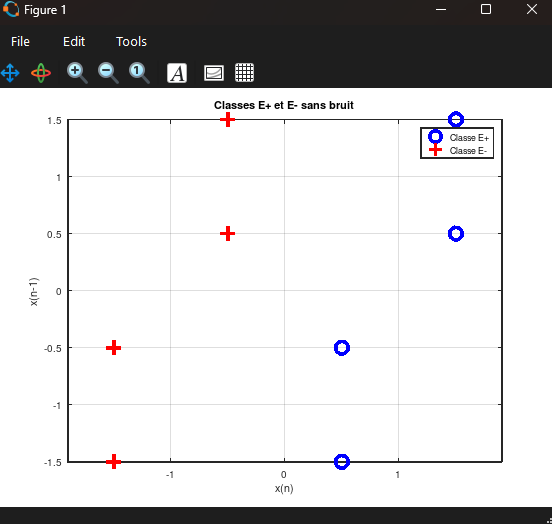
\includegraphics[width=0.82\textwidth]{../figures/01_classes_sans_bruit.png}
}{
    \fbox{\parbox{0.78\textwidth}{\centering Figure à ajouter : \texttt{01\_classes\_sans\_bruit.png}}}
}
\caption{Représentation des motifs des classes $E^+$ et $E^-$ sans bruit.}
\label{fig:yassine-sans-bruit}
\end{figure}

La figure~\ref{fig:yassine-sans-bruit} présente les huit motifs théoriques calculés à partir de la matrice $CC$. Chaque point correspond à une combinaison des trois symboles $d(n)$, $d(n-1)$ et $d(n-2)$. En absence de bruit, les observations prennent exactement les coordonnées calculées dans les tableaux précédents : aucune dispersion aléatoire n'est présente.

Cette figure constitue la référence pour l'étude du bruit. Elle permet de comparer les positions idéales des motifs avec les observations perturbées dans les expériences suivantes.

\subsection{Modélisation du bruit gaussien}

Nous ajoutons aux observations un bruit gaussien centré :
\[
W(n)\sim\mathcal{N}(0,\sigma^2 I_P),
\]
où $\sigma^2$ est la variance du bruit et $I_P$ la matrice identité de dimension $P$.

Les observations bruitées s'écrivent :
\begin{equation}
X_{\mathrm{bruité}}(n)=CC\,D(n)+W(n).
\end{equation}

Dans le programme Octave, les composantes du bruit sont générées avec \texttt{randn}, puis multipliées par $\sqrt{\sigma^2}$ afin d'obtenir la variance souhaitée. La simulation utilise $N=100$ observations par motif. Les variances $0.01$, $0.2$ et $1.0$ sont des valeurs choisies pour illustrer l'effet progressif du bruit ; elles ne constituent pas des valeurs imposées par l'énoncé.

\subsection{Analyse des résultats avec bruit}

\begin{figure}[H]
\centering
\IfFileExists{../figures/02_classes_bruit_variance_0_01.png}{
    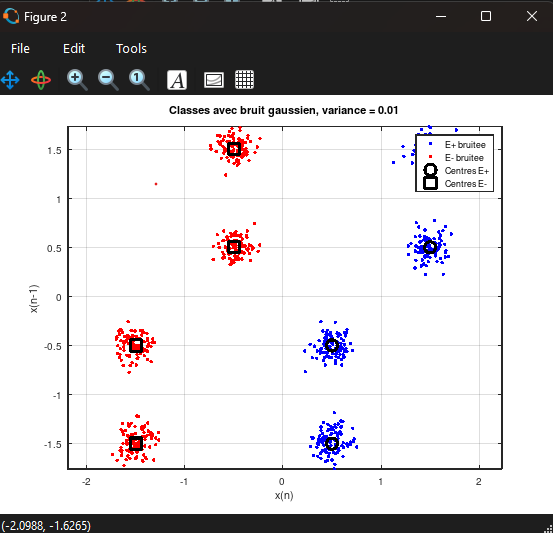
\includegraphics[width=0.82\textwidth]{../figures/02_classes_bruit_variance_0_01.png}
}{
    \fbox{\parbox{0.78\textwidth}{\centering Figure à ajouter : \texttt{02\_classes\_bruit\_variance\_0\_01.png}}}
}
\caption{Observations bruitées pour une variance $\sigma^2=0.01$.}
\label{fig:yassine-bruit-faible}
\end{figure}

Pour $\sigma^2=0.01$, le bruit est faible. Les observations restent généralement proches des positions théoriques de la figure~\ref{fig:yassine-sans-bruit}. La dispersion autour des motifs est limitée et les deux classes conservent une séparation visuelle nette. Le bruit modifie légèrement les coordonnées, sans perturber fortement la structure des classes.

\begin{figure}[H]
\centering
\IfFileExists{../figures/03_classes_bruit_variance_0_2.png}{
    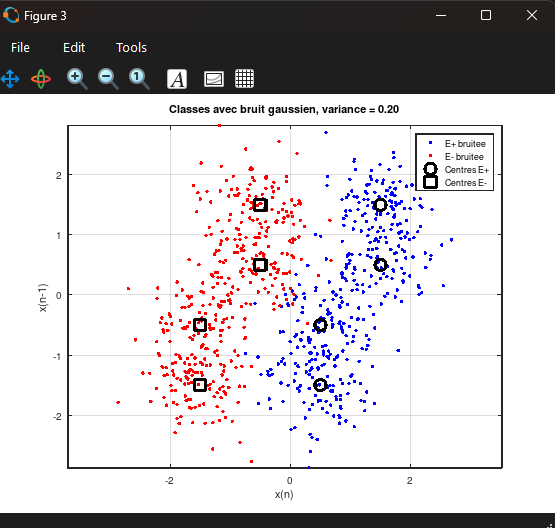
\includegraphics[width=0.82\textwidth]{../figures/03_classes_bruit_variance_0_2.png}
}{
    \fbox{\parbox{0.78\textwidth}{\centering Figure à ajouter : \texttt{03\_classes\_bruit\_variance\_0\_2.png}}}
}
\caption{Observations bruitées pour une variance $\sigma^2=0.2$.}
\label{fig:yassine-bruit-moyen}
\end{figure}

Lorsque la variance augmente à $\sigma^2=0.2$, l'amplitude typique des perturbations devient plus importante. Les nuages de points sont davantage étalés autour des motifs théoriques. La distinction entre les classes est donc moins évidente que dans le cas du bruit faible, même si les observations restent globalement organisées autour de leurs positions théoriques.

\begin{figure}[H]
\centering
\IfFileExists{../figures/04_classes_bruit_variance_1_0.png}{
    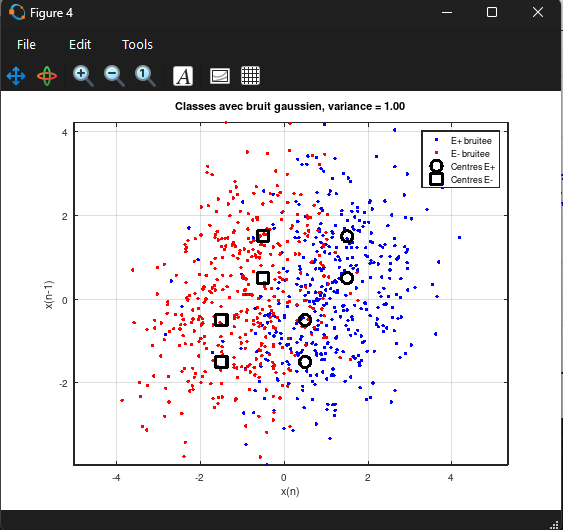
\includegraphics[width=0.82\textwidth]{../figures/04_classes_bruit_variance_1_0.png}
}{
    \fbox{\parbox{0.78\textwidth}{\centering Figure à ajouter : \texttt{04\_classes\_bruit\_variance\_1\_0.png}}}
}
\caption{Observations bruitées pour une variance $\sigma^2=1.0$.}
\label{fig:yassine-bruit-fort}
\end{figure}

Pour $\sigma^2=1.0$, le bruit est important. Les observations peuvent s'éloigner sensiblement de leurs positions théoriques et les nuages deviennent plus dispersés. Des observations appartenant à des classes différentes peuvent alors se rapprocher, voire se chevaucher localement. La distinction entre les classes devient plus difficile et le risque d'erreur de classification augmente.

\begin{figure}[H]
\centering
\IfFileExists{../figures/05_comparaison_niveaux_bruit.png}{
    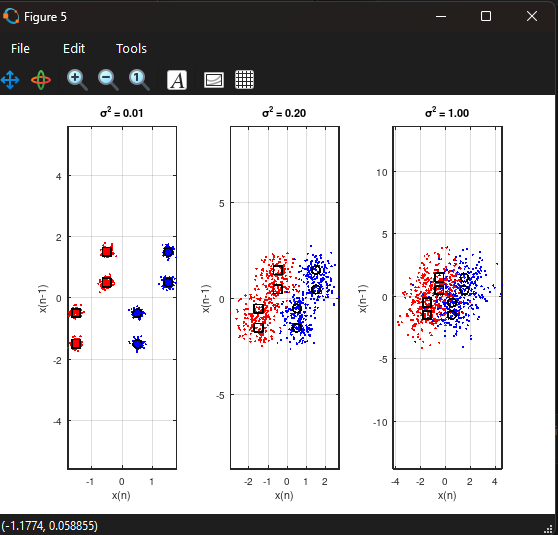
\includegraphics[width=0.90\textwidth]{../figures/05_comparaison_niveaux_bruit.png}
}{
    \fbox{\parbox{0.82\textwidth}{\centering Figure à ajouter : \texttt{05\_comparaison\_niveaux\_bruit.png}}}
}
\caption{Comparaison des observations pour les trois niveaux de bruit étudiés.}
\label{fig:yassine-comparaison-bruit}
\end{figure}

La comparaison met en évidence l'effet direct de la variance sur la dispersion des observations. Lorsque $\sigma^2$ augmente, les points s'écartent davantage de leurs positions idéales. La séparation visuelle des classes se dégrade progressivement, ce qui explique pourquoi une classification fiable devient plus difficile en présence d'un bruit important.

\subsection{Bilan de la partie 1.1}

La matrice de convolution $CC$ permet de représenter l'effet du canal sur les symboles transmis. Pour $M=2$ et $P=2$, les deux valeurs possibles du symbole courant définissent deux classes, et les deux symboles précédents conduisent à quatre motifs par classe.

Sans bruit, les motifs occupent leurs positions théoriques. L'ajout d'un bruit gaussien entraîne une dispersion autour de ces positions. Les simulations montrent que cette dispersion augmente avec la variance du bruit et peut rendre les classes plus difficiles à distinguer. Cette observation justifie l'intérêt d'un classifieur capable de prendre en compte les distributions statistiques des observations, comme le classifieur bayésien étudié dans la suite du TP.

\section{DiffWave : critère d'apprentissage, latence et mémoire}

\subsection{Principe général}

DiffWave est un modèle génératif fondé sur la diffusion, conçu pour produire des formes d'onde audio. Le processus direct ajoute progressivement du bruit à un signal audio réel jusqu'à obtenir un signal proche d'un bruit gaussien. Le processus inverse apprend à retirer progressivement ce bruit afin de reconstruire un signal audio plausible.

Pendant l'apprentissage, le réseau est entraîné sur des signaux perturbés à différents niveaux de diffusion. Il reçoit le signal bruité et l'indice de l'étape de diffusion, puis apprend à estimer le bruit qui a été ajouté.

\subsection{Critère de coût utilisé pendant l'apprentissage}

Une formulation courante de l'objectif d'apprentissage consiste à minimiser l'erreur quadratique entre le bruit réellement ajouté et le bruit estimé par le réseau :
\begin{equation}
\mathcal{L}(\theta)=
\mathbb{E}_{x_0,\epsilon,t}
\left[
\left\|
\epsilon-\epsilon_\theta(x_t,t)
\right\|_2^2
\right],
\end{equation}
où :
\begin{itemize}
    \item $x_0$ est le signal audio original ;
    \item $t$ est l'indice de l'étape de diffusion ;
    \item $\epsilon$ est le bruit gaussien ajouté ;
    \item $x_t$ est le signal perturbé à l'étape $t$ ;
    \item $\epsilon_\theta(x_t,t)$ est le bruit prédit par le réseau paramétré par $\theta$.
\end{itemize}

Le réseau cherche à produire une estimation du bruit aussi proche que possible du bruit réellement injecté. En apprenant à estimer ce bruit à différents niveaux de perturbation, il apprend indirectement à effectuer le processus inverse de diffusion.

L'article original de DiffWave présente un cadre probabiliste de diffusion et un objectif d'apprentissage lié à la borne variationnelle. La prédiction du bruit avec une erreur quadratique est une formulation pratique couramment utilisée pour entraîner ce type de modèle. Cette fonction de coût ne mesure pas directement la qualité audio finale : elle mesure l'écart entre le bruit réel et le bruit estimé pendant l'apprentissage.

\subsection{Latence et temps de génération}

La latence désigne le temps nécessaire pour générer le signal audio. Dans un modèle de diffusion, la génération nécessite plusieurs étapes successives du processus inverse. À chaque étape, le réseau estime le bruit et permet de produire un signal progressivement plus structuré.

Le temps de génération dépend principalement :
\begin{itemize}
    \item du nombre d'étapes de diffusion utilisées pendant l'inférence ;
    \item de la longueur du signal audio à générer ;
    \item de la taille et de la complexité du réseau ;
    \item du matériel utilisé, notamment du processeur ou du GPU ;
    \item de l'optimisation logicielle et de la précision numérique.
\end{itemize}

DiffWave est non autorégressif : il n'a pas besoin de prédire chaque échantillon audio en s'appuyant séquentiellement sur les échantillons précédents, comme le font les modèles autorégressifs classiques. Les opérations sur les positions temporelles d'une étape peuvent être réalisées en parallèle. En revanche, les étapes successives du processus inverse de diffusion restent dépendantes les unes des autres.

Augmenter le nombre d'étapes de diffusion peut améliorer la qualité de la génération, mais augmente généralement le temps de calcul. Il existe donc un compromis entre qualité audio et latence. Une valeur précise doit être mesurée sur une machine et avec une configuration données ; aucune mesure locale n'est avancée dans ce rapport.

\subsection{Consommation mémoire}

La consommation mémoire correspond à la quantité de mémoire vive ou de mémoire GPU nécessaire au chargement et à l'exécution du modèle. Elle dépend notamment :
\begin{itemize}
    \item du nombre de paramètres du réseau ;
    \item du nombre de canaux et de blocs internes de l'architecture ;
    \item de la longueur des séquences audio traitées ;
    \item de la taille du lot (\textit{batch size}) ;
    \item de la précision numérique utilisée ;
    \item du mode d'exécution : apprentissage ou inférence.
\end{itemize}

Pendant l'apprentissage, la consommation mémoire est généralement plus importante, car il faut conserver les activations intermédiaires nécessaires à la rétropropagation du gradient, en plus des paramètres et des états de l'optimiseur.

Pendant l'inférence, le calcul du gradient n'est pas nécessaire. La mémoire requise est donc généralement plus faible, même si elle reste influencée par la taille du modèle et la longueur audio générée.

Il faut distinguer la taille du fichier contenant les poids pré-entraînés de la mémoire réellement utilisée à l'exécution. Le chargement du modèle, les activations intermédiaires, les tampons de calcul et les données audio peuvent nécessiter davantage de mémoire que le seul fichier des poids.

\subsection{Synthèse de l'étude de DiffWave}

Le critère d'apprentissage de DiffWave vise à rapprocher le bruit prédit par le réseau du bruit réellement ajouté au signal. La latence dépend notamment du nombre d'étapes de diffusion, de la longueur audio et du matériel disponible. La mémoire dépend de l'architecture, des dimensions des données et du mode d'exécution.

Ces trois critères sont liés : une configuration plus coûteuse en calcul ou en mémoire peut permettre une génération de meilleure qualité, mais elle peut aussi augmenter les ressources nécessaires. L'évaluation pratique d'un modèle DiffWave doit donc considérer simultanément la qualité audio, le temps de génération et la consommation mémoire.

\section*{Conclusion de la partie}
\addcontentsline{toc}{section}{Conclusion de la partie de Yassine}

La première étude a permis de construire les motifs des deux classes à partir de la matrice de convolution et d'observer l'influence du bruit gaussien sur leur séparation. Les figures montrent que l'augmentation de la variance entraîne une dispersion plus importante des observations et complique progressivement la classification.

L'étude de DiffWave a permis de comprendre le rôle du critère de prédiction du bruit pendant l'apprentissage, ainsi que les principaux facteurs qui influencent la latence et la consommation mémoire du modèle.





% Ne pas ajouter de \documentclass, \begin{document} ou \end{document} ici.

\chapter{Motifs des classes et étude de DiffWave}

\section{Construction des motifs des classes}

\subsection{Objectif et modèle du signal}

L'objectif de cette partie est de construire les deux classes de symboles, notées $E^+$ et $E^-$, puis d'étudier leur représentation dans l'espace des observations. Le symbole courant prend l'une des deux valeurs :
\[
d(n)\in\{-1,+1\}.
\]

Le signal reçu est modélisé par la convolution du signal transmis avec la réponse impulsionnelle du canal, à laquelle s'ajoute un bruit :
\begin{equation}
x(n)=\sum_{i=0}^{M-1}c(i)d(n-i)+w(n),
\end{equation}
où $c(i)$ représente les coefficients du canal, $d(n)$ les symboles transmis et $w(n)$ le bruit additif.

Les paramètres utilisés sont :
\[
M=2,\qquad P=2,\qquad c(0)=1,\qquad c(1)=0.5.
\]
Le vecteur d'observation contient deux échantillons successifs :
\[
X(n)=
\begin{pmatrix}
x(n)\\
x(n-1)
\end{pmatrix}.
\]

\subsection{Construction de la matrice de convolution}

Pour calculer les deux composantes de $X(n)$, nous considérons le vecteur des symboles :
\[
D(n)=
\begin{pmatrix}
d(n)\\
d(n-1)\\
d(n-2)
\end{pmatrix}.
\]

En absence de bruit, la relation matricielle s'écrit :
\begin{equation}
X(n)=CC\,D(n),
\end{equation}
avec :
\begin{equation}
CC=
\begin{pmatrix}
c(0)&c(1)&0\\
0&c(0)&c(1)
\end{pmatrix}
=
\begin{pmatrix}
1&0.5&0\\
0&1&0.5
\end{pmatrix}.
\end{equation}

La première ligne donne $x(n)=d(n)+0.5d(n-1)$, tandis que la deuxième donne $x(n-1)=d(n-1)+0.5d(n-2)$. La matrice $CC$ traduit donc l'effet du canal sur les symboles courant et passés.

\subsection{Détermination des quatre motifs de chaque classe}

La classe $E^+$ correspond à $d(n)=+1$ et la classe $E^-$ à $d(n)=-1$. Les deux symboles précédents, $d(n-1)$ et $d(n-2)$, peuvent chacun prendre les valeurs $-1$ ou $+1$. Il existe donc $2^2=4$ combinaisons par classe, soit huit motifs au total.

Les coordonnées sont calculées à partir de $X(n)=CC\,D(n)$.

\begin{table}[H]
\centering
\caption{Motifs théoriques de la classe $E^+$ sans bruit}
\label{tab:yassine-motifs-plus}
\begin{tabular}{ccccc}
\toprule
$d(n)$ & $d(n-1)$ & $d(n-2)$ & $x(n)$ & $x(n-1)$\\
\midrule
$+1$ & $+1$ & $+1$ & $1.5$ & $1.5$\\
$+1$ & $+1$ & $-1$ & $1.5$ & $0.5$\\
$+1$ & $-1$ & $+1$ & $0.5$ & $-0.5$\\
$+1$ & $-1$ & $-1$ & $0.5$ & $-1.5$\\
\bottomrule
\end{tabular}
\end{table}

\begin{table}[H]
\centering
\caption{Motifs théoriques de la classe $E^-$ sans bruit}
\label{tab:yassine-motifs-moins}
\begin{tabular}{ccccc}
\toprule
$d(n)$ & $d(n-1)$ & $d(n-2)$ & $x(n)$ & $x(n-1)$\\
\midrule
$-1$ & $+1$ & $+1$ & $-0.5$ & $1.5$\\
$-1$ & $+1$ & $-1$ & $-0.5$ & $0.5$\\
$-1$ & $-1$ & $+1$ & $-1.5$ & $-0.5$\\
$-1$ & $-1$ & $-1$ & $-1.5$ & $-1.5$\\
\bottomrule
\end{tabular}
\end{table}

\subsection{Résultats en absence de bruit}

\begin{figure}[H]
\centering
\IfFileExists{../figures/01_classes_sans_bruit.png}{
    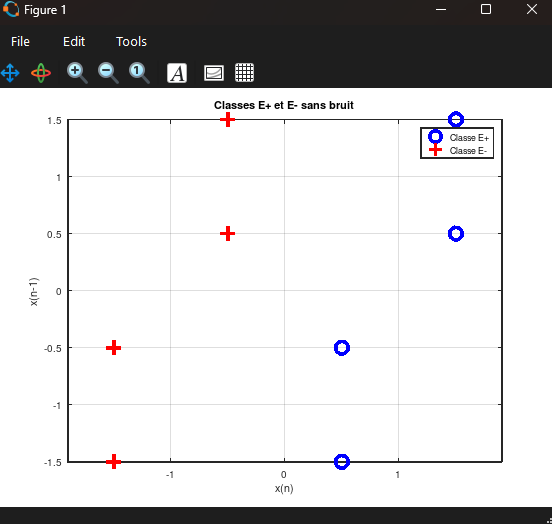
\includegraphics[width=0.82\textwidth]{../figures/01_classes_sans_bruit.png}
}{
    \fbox{\parbox{0.78\textwidth}{\centering Figure à ajouter : \texttt{01\_classes\_sans\_bruit.png}}}
}
\caption{Représentation des motifs des classes $E^+$ et $E^-$ sans bruit.}
\label{fig:yassine-sans-bruit}
\end{figure}

La figure~\ref{fig:yassine-sans-bruit} présente les huit motifs théoriques calculés à partir de la matrice $CC$. Chaque point correspond à une combinaison des trois symboles $d(n)$, $d(n-1)$ et $d(n-2)$. En absence de bruit, les observations prennent exactement les coordonnées calculées dans les tableaux précédents : aucune dispersion aléatoire n'est présente.

Cette figure constitue la référence pour l'étude du bruit. Elle permet de comparer les positions idéales des motifs avec les observations perturbées dans les expériences suivantes.

\subsection{Modélisation du bruit gaussien}

Nous ajoutons aux observations un bruit gaussien centré :
\[
W(n)\sim\mathcal{N}(0,\sigma^2 I_P),
\]
où $\sigma^2$ est la variance du bruit et $I_P$ la matrice identité de dimension $P$.

Les observations bruitées s'écrivent :
\begin{equation}
X_{\mathrm{bruité}}(n)=CC\,D(n)+W(n).
\end{equation}

Dans le programme Octave, les composantes du bruit sont générées avec \texttt{randn}, puis multipliées par $\sqrt{\sigma^2}$ afin d'obtenir la variance souhaitée. La simulation utilise $N=100$ observations par motif. Les variances $0.01$, $0.2$ et $1.0$ sont des valeurs choisies pour illustrer l'effet progressif du bruit ; elles ne constituent pas des valeurs imposées par l'énoncé.

\subsection{Analyse des résultats avec bruit}

\begin{figure}[H]
\centering
\IfFileExists{../figures/02_classes_bruit_variance_0_01.png}{
    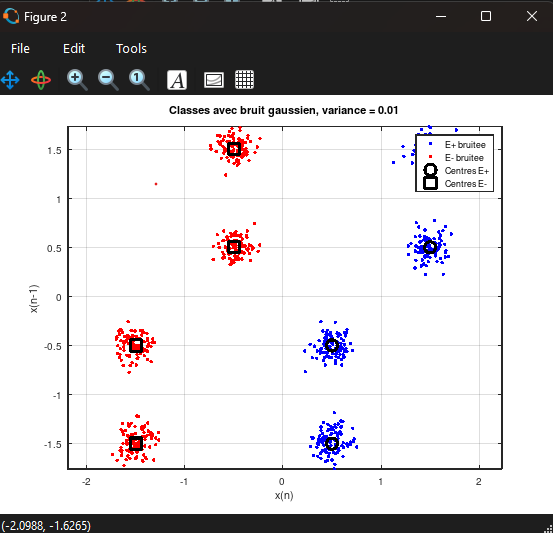
\includegraphics[width=0.82\textwidth]{../figures/02_classes_bruit_variance_0_01.png}
}{
    \fbox{\parbox{0.78\textwidth}{\centering Figure à ajouter : \texttt{02\_classes\_bruit\_variance\_0\_01.png}}}
}
\caption{Observations bruitées pour une variance $\sigma^2=0.01$.}
\label{fig:yassine-bruit-faible}
\end{figure}

Pour $\sigma^2=0.01$, le bruit est faible. Les observations restent généralement proches des positions théoriques de la figure~\ref{fig:yassine-sans-bruit}. La dispersion autour des motifs est limitée et les deux classes conservent une séparation visuelle nette. Le bruit modifie légèrement les coordonnées, sans perturber fortement la structure des classes.

\begin{figure}[H]
\centering
\IfFileExists{../figures/03_classes_bruit_variance_0_2.png}{
    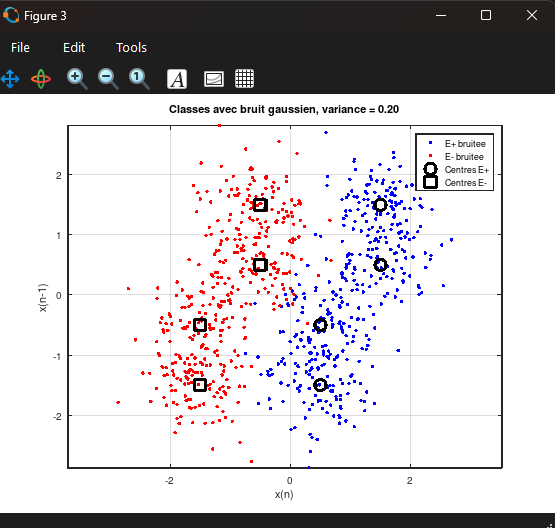
\includegraphics[width=0.82\textwidth]{../figures/03_classes_bruit_variance_0_2.png}
}{
    \fbox{\parbox{0.78\textwidth}{\centering Figure à ajouter : \texttt{03\_classes\_bruit\_variance\_0\_2.png}}}
}
\caption{Observations bruitées pour une variance $\sigma^2=0.2$.}
\label{fig:yassine-bruit-moyen}
\end{figure}

Lorsque la variance augmente à $\sigma^2=0.2$, l'amplitude typique des perturbations devient plus importante. Les nuages de points sont davantage étalés autour des motifs théoriques. La distinction entre les classes est donc moins évidente que dans le cas du bruit faible, même si les observations restent globalement organisées autour de leurs positions théoriques.

\begin{figure}[H]
\centering
\IfFileExists{../figures/04_classes_bruit_variance_1_0.png}{
    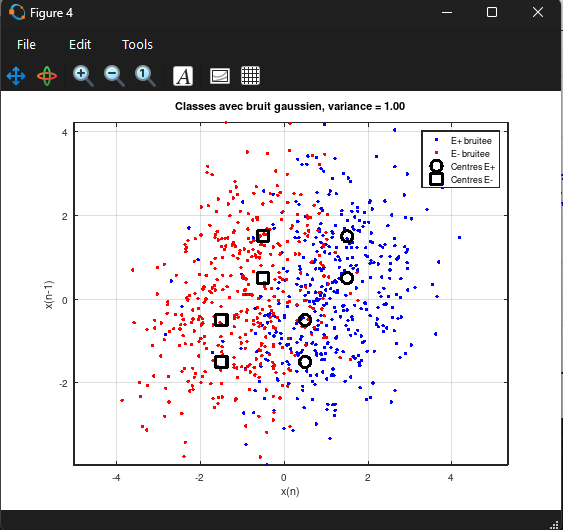
\includegraphics[width=0.82\textwidth]{../figures/04_classes_bruit_variance_1_0.png}
}{
    \fbox{\parbox{0.78\textwidth}{\centering Figure à ajouter : \texttt{04\_classes\_bruit\_variance\_1\_0.png}}}
}
\caption{Observations bruitées pour une variance $\sigma^2=1.0$.}
\label{fig:yassine-bruit-fort}
\end{figure}

Pour $\sigma^2=1.0$, le bruit est important. Les observations peuvent s'éloigner sensiblement de leurs positions théoriques et les nuages deviennent plus dispersés. Des observations appartenant à des classes différentes peuvent alors se rapprocher, voire se chevaucher localement. La distinction entre les classes devient plus difficile et le risque d'erreur de classification augmente.

\begin{figure}[H]
\centering
\IfFileExists{../figures/05_comparaison_niveaux_bruit.png}{
    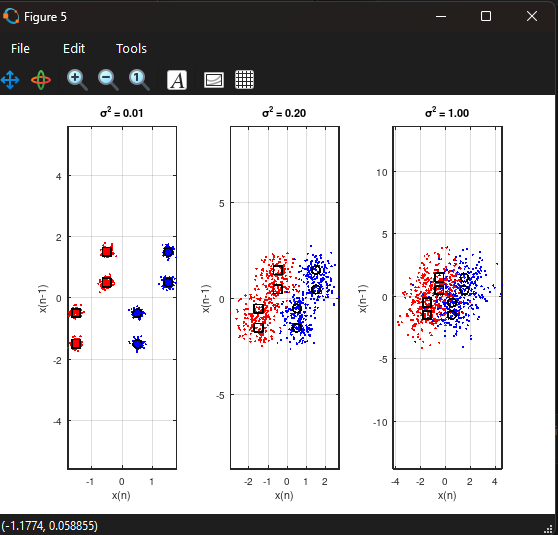
\includegraphics[width=0.90\textwidth]{../figures/05_comparaison_niveaux_bruit.png}
}{
    \fbox{\parbox{0.82\textwidth}{\centering Figure à ajouter : \texttt{05\_comparaison\_niveaux\_bruit.png}}}
}
\caption{Comparaison des observations pour les trois niveaux de bruit étudiés.}
\label{fig:yassine-comparaison-bruit}
\end{figure}

La comparaison met en évidence l'effet direct de la variance sur la dispersion des observations. Lorsque $\sigma^2$ augmente, les points s'écartent davantage de leurs positions idéales. La séparation visuelle des classes se dégrade progressivement, ce qui explique pourquoi une classification fiable devient plus difficile en présence d'un bruit important.

\subsection{Bilan de la partie 1.1}

La matrice de convolution $CC$ permet de représenter l'effet du canal sur les symboles transmis. Pour $M=2$ et $P=2$, les deux valeurs possibles du symbole courant définissent deux classes, et les deux symboles précédents conduisent à quatre motifs par classe.

Sans bruit, les motifs occupent leurs positions théoriques. L'ajout d'un bruit gaussien entraîne une dispersion autour de ces positions. Les simulations montrent que cette dispersion augmente avec la variance du bruit et peut rendre les classes plus difficiles à distinguer. Cette observation justifie l'intérêt d'un classifieur capable de prendre en compte les distributions statistiques des observations, comme le classifieur bayésien étudié dans la suite du TP.

\section{DiffWave : critère d'apprentissage, latence et mémoire}

\subsection{Principe général}

DiffWave est un modèle génératif fondé sur la diffusion, conçu pour produire des formes d'onde audio. Le processus direct ajoute progressivement du bruit à un signal audio réel jusqu'à obtenir un signal proche d'un bruit gaussien. Le processus inverse apprend à retirer progressivement ce bruit afin de reconstruire un signal audio plausible.

Pendant l'apprentissage, le réseau est entraîné sur des signaux perturbés à différents niveaux de diffusion. Il reçoit le signal bruité et l'indice de l'étape de diffusion, puis apprend à estimer le bruit qui a été ajouté.

\subsection{Critère de coût utilisé pendant l'apprentissage}

Une formulation courante de l'objectif d'apprentissage consiste à minimiser l'erreur quadratique entre le bruit réellement ajouté et le bruit estimé par le réseau :
\begin{equation}
\mathcal{L}(\theta)=
\mathbb{E}_{x_0,\epsilon,t}
\left[
\left\|
\epsilon-\epsilon_\theta(x_t,t)
\right\|_2^2
\right],
\end{equation}
où :
\begin{itemize}
    \item $x_0$ est le signal audio original ;
    \item $t$ est l'indice de l'étape de diffusion ;
    \item $\epsilon$ est le bruit gaussien ajouté ;
    \item $x_t$ est le signal perturbé à l'étape $t$ ;
    \item $\epsilon_\theta(x_t,t)$ est le bruit prédit par le réseau paramétré par $\theta$.
\end{itemize}

Le réseau cherche à produire une estimation du bruit aussi proche que possible du bruit réellement injecté. En apprenant à estimer ce bruit à différents niveaux de perturbation, il apprend indirectement à effectuer le processus inverse de diffusion.

L'article original de DiffWave présente un cadre probabiliste de diffusion et un objectif d'apprentissage lié à la borne variationnelle. La prédiction du bruit avec une erreur quadratique est une formulation pratique couramment utilisée pour entraîner ce type de modèle. Cette fonction de coût ne mesure pas directement la qualité audio finale : elle mesure l'écart entre le bruit réel et le bruit estimé pendant l'apprentissage.

\subsection{Latence et temps de génération}

La latence désigne le temps nécessaire pour générer le signal audio. Dans un modèle de diffusion, la génération nécessite plusieurs étapes successives du processus inverse. À chaque étape, le réseau estime le bruit et permet de produire un signal progressivement plus structuré.

Le temps de génération dépend principalement :
\begin{itemize}
    \item du nombre d'étapes de diffusion utilisées pendant l'inférence ;
    \item de la longueur du signal audio à générer ;
    \item de la taille et de la complexité du réseau ;
    \item du matériel utilisé, notamment du processeur ou du GPU ;
    \item de l'optimisation logicielle et de la précision numérique.
\end{itemize}

DiffWave est non autorégressif : il n'a pas besoin de prédire chaque échantillon audio en s'appuyant séquentiellement sur les échantillons précédents, comme le font les modèles autorégressifs classiques. Les opérations sur les positions temporelles d'une étape peuvent être réalisées en parallèle. En revanche, les étapes successives du processus inverse de diffusion restent dépendantes les unes des autres.

Augmenter le nombre d'étapes de diffusion peut améliorer la qualité de la génération, mais augmente généralement le temps de calcul. Il existe donc un compromis entre qualité audio et latence. Une valeur précise doit être mesurée sur une machine et avec une configuration données ; aucune mesure locale n'est avancée dans ce rapport.

\subsection{Consommation mémoire}

La consommation mémoire correspond à la quantité de mémoire vive ou de mémoire GPU nécessaire au chargement et à l'exécution du modèle. Elle dépend notamment :
\begin{itemize}
    \item du nombre de paramètres du réseau ;
    \item du nombre de canaux et de blocs internes de l'architecture ;
    \item de la longueur des séquences audio traitées ;
    \item de la taille du lot (\textit{batch size}) ;
    \item de la précision numérique utilisée ;
    \item du mode d'exécution : apprentissage ou inférence.
\end{itemize}

Pendant l'apprentissage, la consommation mémoire est généralement plus importante, car il faut conserver les activations intermédiaires nécessaires à la rétropropagation du gradient, en plus des paramètres et des états de l'optimiseur.

Pendant l'inférence, le calcul du gradient n'est pas nécessaire. La mémoire requise est donc généralement plus faible, même si elle reste influencée par la taille du modèle et la longueur audio générée.

Il faut distinguer la taille du fichier contenant les poids pré-entraînés de la mémoire réellement utilisée à l'exécution. Le chargement du modèle, les activations intermédiaires, les tampons de calcul et les données audio peuvent nécessiter davantage de mémoire que le seul fichier des poids.

\subsection{Synthèse de l'étude de DiffWave}

Le critère d'apprentissage de DiffWave vise à rapprocher le bruit prédit par le réseau du bruit réellement ajouté au signal. La latence dépend notamment du nombre d'étapes de diffusion, de la longueur audio et du matériel disponible. La mémoire dépend de l'architecture, des dimensions des données et du mode d'exécution.

Ces trois critères sont liés : une configuration plus coûteuse en calcul ou en mémoire peut permettre une génération de meilleure qualité, mais elle peut aussi augmenter les ressources nécessaires. L'évaluation pratique d'un modèle DiffWave doit donc considérer simultanément la qualité audio, le temps de génération et la consommation mémoire.

\section*{Conclusion de la partie}
\addcontentsline{toc}{section}{Conclusion de la partie de Yassine}

La première étude a permis de construire les motifs des deux classes à partir de la matrice de convolution et d'observer l'influence du bruit gaussien sur leur séparation. Les figures montrent que l'augmentation de la variance entraîne une dispersion plus importante des observations et complique progressivement la classification.

L'étude de DiffWave a permis de comprendre le rôle du critère de prédiction du bruit pendant l'apprentissage, ainsi que les principaux facteurs qui influencent la latence et la consommation mémoire du modèle.





\section{seif}
\section{raslen}


\end{document}